\chapter{DCE in a Periodic Potential} \label{ch:system}


\section{Circuit analysis for a 1D periodic potential quantum network}\label{sec:circ_an}
%
\color{blue}
\noindent
We now proceed to the study of the DCE in our proposed system, which consists of a periodic array of CPWs connected by SQUIDs (see Fig. \ref{fig:circuit_diagram}) . We employ a field-theoretic description of the system, we discretize by breaking it up into segments $i$ of length $\Delta x$ with capacitance $\Delta x \, C_0$, inductance $\Delta x \, L_0$, and dynamical fluxes $\Phi_i(t)$ (see Ch.\ref{sec:SC_and_SQUIDs}).
Assuming symmetric SQUIDs, the Lagrangian for this system is (cp. Johansson \cite{Johansson2010_DCE}, Eq.\,(5))
\color{red} \{note edits: use index $n$ for SQUIDs instead of $s$\} \color{blue}
%
\begin{figure}[h]\label{fig:circuit_diagram}
    %Hand-drawn placeholder figures. Made to work out placement, size, and captions while high resolution figures are generated.
    \centering
    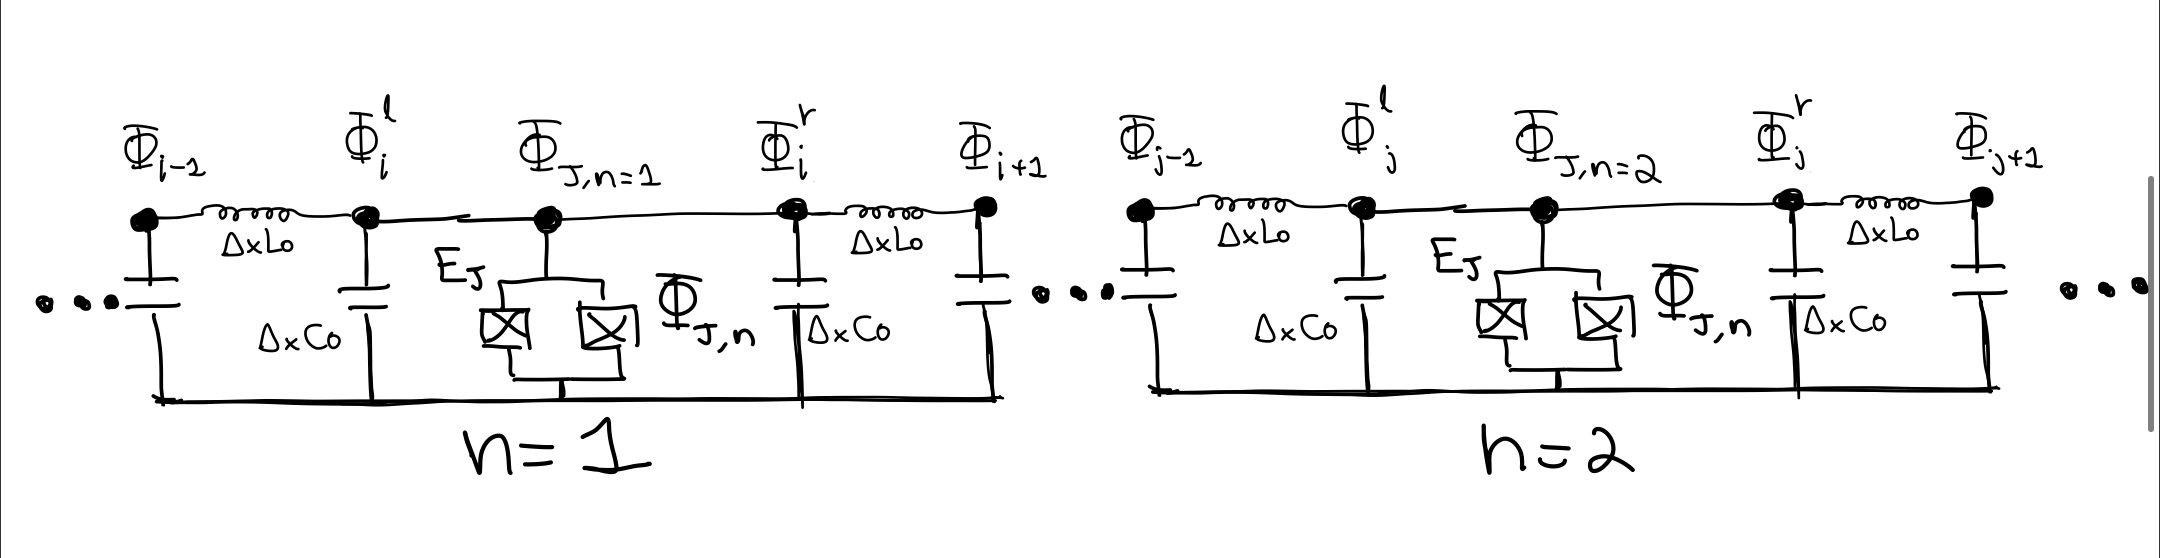
\includegraphics[width=\textwidth, keepaspectratio]{figures/circuit_diagram.png}
    \caption{Circuit diagram for a periodic lattice consisting of CPWs connected by symmetric SQUIDs at lattice sites $n$. The dynamical fluxes $\Phi_i$ and $\Phi_{J,n}$ characterize the system.}
\end{figure}
%
\begin{equation} \label{eq:lagn1}
\begin{split}
\mathcal{L} = \, & \frac{1}{2} \sum_i \left( \Delta x \, C_{0} \left(\dot{\Phi}_{i}\right)^{2} \, - \, 
\frac{\left(\Phi_{i+1}-\Phi_{i}\right)^{2}}{\Delta x \, L_{0}} \right)  \\[2mm]
& + \sum_n \left[ \frac{1}{2} \, C_{J,\,n} \left(\dot{\Phi}_{J,\,n} \right)^{2} \, + \, 
E_{J,\,n}(t) \cos\left(2\pi \frac{\Phi_{J,\,n}}{\Phi_0} \right) \right]
\end{split}
\end{equation}
%
where a dot over a symbol indicates a time derivative, e.g., 
$\displaystyle \dot{\Phi}_i = \frac{\partial}{\partial t} \Phi_i$.
The terms on the r.h.s.\,of the first line of Eq.\,(\ref{eq:lagn1}) describe sections of the CPW between the SQUIDs. 
The second line of Eq.\,(\ref{eq:lagn1}) describes a periodic array of SQUIDs indexed by $n$ 
with effective capacitance $C_{J,\,n}$ and flux $\Phi_{J,\,n}$ at node $n$, where 
the subscript $J$ stands for the two Josephson junctions of a SQUID.
$\Phi_0 = h / (2 e)$ is the magnetic flux quantum.
The SQUIDs are separated by 
distance $\ell$ corresponding to the lattice constant of the one-dimensional (1D) SQUID array. 
The Josephson energy $E_{J,\,n}(t)$ of SQUID $n$ is tunable
by the externally applied magnetic flux $\Phi_{\text{ext},\,n}(t)$ through the SQUID 
(cp. Johansson, Eq.\,(6)): 
%
\begin{equation} \label{eq:squidenergy}
    E_{J,\,n}(t) = 2 \, \epsilon_{J,\,n} 
    \left\vert \cos\left(\pi \, \frac{\Phi_{\text{ext},\,n}(t)}{\Phi_0}\right)\right\vert \, \, ,
\end{equation}
%
where $\epsilon_{J,\,n}$ is a constant energy parameter.

We assume that the plasma frequency $\omega_p$ of the SQUIDs far exceeds other characteristic frequencies 
in the circuit so that oscillations in the phase across the SQUIDs have small amplitude, i.e., 
$\Phi_{J,\,n} / \Phi_0 \ll 1$,
and the SQUIDs are operated in the phase regime where $E_{J,\,n} \gg (2e)^2 / (2C_{J,\,n})$. 
Using $\Phi_{J,\,n} / \Phi_0 \ll 1$ one may expand the cosine in Eq.\,(\ref{eq:lagn1}), 
resulting in a Lagrangian quadratic in $\Phi_{J,\,n}$ (dropping terms $E_{J,\,n}(t)$ 
independent of $\Phi_{J,\,n}$)
%
\begin{equation} \label{eq:lagn2}
\begin{split}
\mathcal{L} = \, & \frac{1}{2} \sum_i \left( \Delta x \, C_{0} \left(\dot{\Phi}_{i}\right)^{2} \, - \, 
\frac{\left(\Phi_{i+1}-\Phi_{i}\right)^{2}}{\Delta x \, L_{0}} \right)  \\[2mm]
& + \frac{1}{2} \sum_n \left( C_{J,\,n} \left(\dot{\Phi}_{J,\,n} \right)^{2} \, - \, 
 \left(\frac{2 \pi}{\Phi_0} \right)^2 E_{J,\,n}(t) \, \left( \Phi_{J,\,n} \right)^2 
\right) \, \, .
\end{split}
\end{equation}
%
Note that we make the identification $\Phi_i^{\,l} = \Phi_{J,\,n} = \Phi_i^{\,r}$ for the flux at SQUID $n$, 
where $\Phi_i^{\,l}$ and $\Phi_i^{\,r}$ are the fluxes at adjacent nodes to the left ($l$) and right ($r$) of 
node $n$, respectively (see Fig. \ref{fig:circuit_diagram}). 


From now on, we assume that the intrinsic device parameters of all SQUIDs are equal, i.e., 
$C_{J,\,n} = C_J$, $\epsilon_{J,\,n} = \epsilon_J$ for all $n$ in Eqs.\,(\ref{eq:lagn2}), (\ref{eq:squidenergy}).  
Moreover, we assume that the SQUID energy $E_{J,\,n}(t)$ in Eq.\,(\ref{eq:squidenergy}) 
can be expanded in a static part plus weak harmonic drive 
(cp. Johansson, text page 6 bottom left)
%
\begin{equation} \label{eq:energyexp1}
E_{J,\,n}(t) = E_J^0 + \delta E_{J,\,n} \cos(\Omega \, t + \varphi_n) 
\end{equation}
%
where $\delta E_{J,\,n} \ll E_J^0$ and $\Omega$ is the frequency of the external drive 
$\Phi_{\text{ext}}(t)$ in Eq.\,(\ref{eq:squidenergy}).
As indicated in Eq.\,(\ref{eq:energyexp1}), we assume that the {\em static} part 
$E_J^0$ of $E_{J,\,n}(t)$ is the same for all SQUIDs (i.e., indepedent of $n$). 
This assumption is crucial for our 
treatment of the {\em static} system (realized by a static applied magnetic flux $\Phi_{\text{ext}}$
for all SQUIDs) as a 1D periodic lattice with period $\ell$. However, the 
time-dependent perturbation in Eq.\,(\ref{eq:energyexp1})
may be modulated along the SQUID array, i.e., may differ for different SQUIDs $n$,
in terms of amplitudes $\delta E_{J,\,n}$ and phases $\varphi_n$.
This allows us to externally control the DCE radiation generated in the SQUID array
by varying the parameters $\delta E_{J,\,n}$ and $\varphi_n$.
However, we will assume for simplicity that the drive frequency 
is the same for all SQUIDs, i.e., $\Omega_n = \Omega$ for all $n$.
That is, we consider an amplitude modulation but no frequency modulation of the 
time-dependent perturbation in Eq.\,(\ref{eq:energyexp1}). 
%
%
%\begin{equation} \label{eq:energyexp2}
%E_{J,\,n}(t) \equiv E_J(t) = E_J^0 + \delta E_J \cos(\Omega \, t) \qquad \text{for all} \, \, \, \, n \, \, . 
%\end{equation}
%
%With these assumptions, the Lagrangian (\ref{eq:lagn2}) takes the form
%
%\begin{equation} \label{eq:lagn3}
%\begin{split}
%\mathcal{L} = \, & \frac{1}{2} \sum_i \left( \Delta x \, C_{0} \left(\dot{\Phi}_{i}\right)^{2} \, - \, 
%\frac{\left(\Phi_{i+1} - \Phi_{i}\right)^{2}}{\Delta x \, L_{0}} \right)  \\[2mm]
%& + \frac{1}{2} \sum_n \left( C_J \left(\dot{\Phi}_{J,\,n} \right)^{2} \, - \, 
% \left(\frac{2 \pi}{\Phi_0} \right)^2 E_{J,\,n}(t) \, \left( \Phi_{J,\,n} \right)^2 
%\right) \, \, .
%\end{split}
%\end{equation}
%
%with $E_{J,\,n}(t)$ from Eq.(\ref{eq:energyexp1}). 

To quantize the system, we first transform the Lagrangian $\mathcal{L}$ in Eq.\,(\ref{eq:lagn2})
into a Hamiltonian $\mathcal{H}$ by a Legendre transformation.
To this end, it is convenient to temporarily consider the fluxes $\Phi_i^{\,l}$, $\Phi_i^{\,r}$, and $\Phi_{J,\,n}$ 
at SQUIDs $n$ as independent dynamic variables (cp.\,remark below Eq.(\ref{eq:lagn2})) and define 
%
\begin{equation} \label{eq:ham1}
\mathcal{H} = \sum_{i} \frac{\partial\mathcal{L}}{\partial\dot{\Phi}_i} \, \dot{\Phi}_i 
\, + \, \sum_{n} \frac{\partial\mathcal{L}}{\partial\dot{\Phi}_{J,\,n}} \, \dot{\Phi}_{J,\,n}
\, - \, \mathcal{L} \, \, , 
\end{equation}
%
resulting in
%
\begin{equation} \label{eq:ham2}
\begin{split}
\mathcal{H} = \, & \frac{1}{2} \sum_i \left( \frac{P_i^{\,2}}{\Delta x \, C_{0}} \, + \, 
\frac{\left(\Phi_{i+1} - \Phi_{i}\right)^{2}}{\Delta x \, L_{0}} \right)  \\[2mm]
& + \frac{1}{2} \sum_n \left( \frac{\left(P_{J,\,n}\right)^2}{C_{J}} \, + \, 
 \left(\frac{2 \pi}{\Phi_0} \right)^2 E_J(t) \, \left( \Phi_{J,\,n} \right)^2 
\right) \, \, .
\end{split}
\end{equation}
%
with the canonical conjugate momenta
%
\begin{subequations} \label{eq:mom}
\begin{eqnarray} 
P_i = \frac{\partial\mathcal{L}}{\partial\dot{\Phi}_i} = \Delta x \, C_0 \, \dot{\Phi}_i \label{eq:moma} \, \, \, , \\[2mm]
P_{J,\,n} = \frac{\partial\mathcal{L}}{\partial\dot{\Phi}_{J,\,n}} =  C_J \, \dot{\Phi}_{J,\,n} \, \, \,  . \label{eq:momb}
\end{eqnarray}
\end{subequations}
%
At this point, we identify again 
$\Phi_i^{\,l} = \Phi_{J,\,n} = \Phi_i^{\,r}$ and $P_i^{\,l} = P_{J,\,n} = P_i^{\,r}$
for the fluxes and conjugate momenta at SQUIDs $n$.
The system is quantized by turning the fluxes $\Phi_i$ and conjugate momenta $P_i$ 
to operators $\hat{\Phi}_i$, $\hat{P}_i$ with equal-time commutation relations
%
\begin{equation} \label{eq:cr} 
\left[\hat{\Phi}_i, \hat{P}_j \right] = i \hbar \delta_{ij} \, \, , \quad 
\left[\hat{\Phi}_i, \hat{\Phi}_j \right] = 0 \, \, , \quad 
\left[\hat{P}_i, \hat{P}_j \right] = 0 \, \, \, , 
\end{equation}
%
where the identifications mentioned above understood; for example, 
$\left[\hat{\Phi}_i^{\,l}, \hat{P}_{J,\,n} \right] = \left[\hat{\Phi}_i^{\,r}, \hat{P}_{J,\,n} \right] = i \hbar$ (see Fig. \ref{fig:circuit_diagram}).

%
In the CPW between the SQUIDs, the Heisenberg equation of motion 
$\displaystyle \frac{d}{dt} \hat{P}_i = \frac{i}{\hbar} \left[\hat{\mathcal{H}}, \hat{P}_i \right]$ 
with results in, using Eqs.\,(\ref{eq:ham2}) - (\ref{eq:cr}), 
%
\begin{equation} \label{eq:eom1}
C_0 L_0 \, \frac{d^2}{dt^2} \hat{\Phi}_i \, = \, 
\frac{1}{(\Delta x)^2} \left(\hat{\Phi}_{i+1} - 2 \hat{\Phi}_i +  \hat{\Phi}_{i-1} \right) \, \, .
\end{equation}
%
In the continuum limit $\Delta x \to 0$ the r.h.s.\,of Eq.\,(\ref{eq:eom1}) becomes
$\displaystyle \frac{\partial^2\hat{\Phi}(x,t)}{\partial x^2}$
and we obtain the massless 1D Klein-Gordon equation 
for the dynamic flux operator $\hat{\Phi}(x,t)$ in the CPW between the SQUIDs,
%
\begin{equation} \label{eq:eom2}
\frac{\partial^2\hat{\Phi}(x,t)}{\partial t^2} - v^2 \, \frac{\partial^2\hat{\Phi}(x,t)}{\partial x^2} = 0 \, \, ,
\end{equation}
%
where $v = 1 / \sqrt{C_0 L_0}$ is the wave propagation speed in the CPW.
We note that, in the continuum limit $\Delta x \to 0$, 
the momentum operator conjugate to $\hat{\Phi}(x,t)$ is given by,
instead of Eq.\,(\ref{eq:moma}), 
%
\begin{equation} \label{eq:mom2} 
\hat{\overline{P}}(x,t) := \frac{\hat{P}_{i}(t)}{\Delta x} = 
C_0 \, \frac{\partial}{\partial t} \hat{\Phi}(x,t)
\end{equation}
%
with equal-time commutation relations
%
\begin{equation} \label{eq:cr2} 
\left[\hat{\Phi}(x,t), \hat{\overline{P}}(x',t) \right] = i \hbar \delta(x - x') \, \, , \quad 
\left[\hat{\Phi}(x,t), \hat{\Phi}(x',t) \right] = 0 \, \, , \quad 
\left[\hat{\overline{P}}(x,t), \hat{\overline{P}}(x',t) \right] = 0 \, \, \, , 
\end{equation}
%
where $\delta(x)$ is the 1D delta function (with units of $1/x$).






\color{black}
Similarly, at the $n$th SQUID site, the Heisenberg equations of motion
$\displaystyle \frac{d}{dt} \hat{P}_{J, n} = \frac{i}{\hbar} \left[\hat{\mathcal{H}}, \hat{P}_{J, n} \right]$ 
with
$\displaystyle \frac{d}{dt} \hat{P}_{J,n} = C_J \, \frac{d^2}{dt^2} \hat{\Phi}_{J, n}$ 
by Eq.\,(\ref{eq:momb}) results in, using Eqs.\,(\ref{eq:ham2}) - (\ref{eq:cr}), 
%
\begin{equation}\label{BC_discrete}
C_{J} \frac{d^2}{dt^2} \hat{\Phi}_{J,n} +\hbar\left(\frac{2 \pi}{\Phi_{0}}\right)^{2} E_{j}(t) \hat{\Phi}_{J, n} -\frac{\hbar}{L_{0}}\left(\frac{\hat{\Phi}_{i+1} - 2 \hat{\Phi}_{J, n} - \hat{\Phi}_{i-1}}{\Delta x}\right)=0.
\end{equation}
%
Which, in the continuum limit $\Delta x \to 0$, results in the boundary condition for $\hat{\Phi}(x, t)$ at the SQUID sites $x = x_n$,
%
\begin{equation}\label{eq:BC_field_orig}
C_{J} \frac{\partial^2 \hat{\Phi}(x_n, t)}{\partial t^2} +\hbar\left(\frac{2 \pi}{\Phi_{0}}\right)^{2} E_{j}(t) \hat{\Phi}(x_n, t) -\frac{\hbar}{L_{0}}\left(\left.\frac{\partial \hat{\Phi}(x, t)}{\partial x}\right|_{x_n^{+}}-\left.\frac{\partial \hat{\Phi}(x,t)}{\partial x}\right|_{x_n^{-}}\right)=0.
\end{equation}

\section{Periodic potential and Kronig-Penney model}\label{sec:Periodic_Potential}
%
\noindent
Let us first consider the background periodic potential in the static case where we apply a DC drive so that the SQUID energy $E_J(t) = E_J^0$ is constant. Following the canonical quantization procedure, 
we turn the classical flux field ${\Phi}_n(x,t)$ 
in compartment $n$ of the periodic array (see Fig. \ref{fig:circuit_diagram})
into a field operator $\hat{\Phi}_n(x,t)$, which is expanded in terms of 
annihilation and creation operators $ \hat{a}_n(k)$ and 
${\hat a}_n^\dagger(k)$:
%
\begin{equation} \label{eq:flux_field_orig}
    \hat{\Phi}_n(x,t) = \sqrt{\frac{\hbar}{2 C_0}} 
    \int_{-\infty}^{\infty}\frac{dk}{2 \pi} \frac{1}{\sqrt{\omega_k}}
    \left\{ \hat{a}_n(k) \psi_k(x)e^{-i \omega(k) \, t} + 
    \hat{a}_n^{\dagger}(k) \psi_k^*(x) e^{i \omega(k) \, t} \right\} \, \, .
\end{equation}
%
The annihilation and creation operators obey the commutation relations
%
\begin{equation} \label{eq:cra_orig}
    \left[ \hat{a}_n(k),{\hat a}_{n'}^\dagger(k') \right] = \delta_{nn'} \, 2 \pi \delta(k - k')
\end{equation}
%
and thus have units of $\text{length}^{1/2}$.
The field expansion in Eq.(\ref{eq:flux_field_orig}) also incorporates Bloch-type functions 
%
\begin{equation} \label{eq:psi1}
\psi_k(x) = e^{i k x} u_k(x) \, \, ,   
\end{equation}
%
where $u_k(x)$ has period $\ell$, i.e., $u_k(x + \ell n) = u_k(x)$ for all integers $n$.
The Bloch functions $\psi_k(x)$ in Eq.\,(\ref{eq:psi1}) are unitless, orthogonal with respect to 
the 1D wave vector $k$, and normalized such that
%
\begin{equation} \label{eq:psi1_norm_orig}
\int_{-\infty}^{\infty} dx \, \psi^*_k(x) \psi_{k'}(x) = 2 \pi \, \delta(k - k') \, \, .
\end{equation}
%
%
The introduction of a periodic potential leads to a Bloch band structure similar to the one for electrons in solid state physics (see section \ref{sec:KP_in_SS}) with energy bands determined by the dispersion relation
\begin{equation}\label{eq:disp_rel}
    \cos{k} = \cos{\omega} + \frac{\lambda}{2\omega}\sin{\omega}
\end{equation}
%
where $\lambda$ is defined as:
%
\begin{equation}\label{eq:lambda}
\lambda = \left(\frac{L_0}{\hbar}\right)  
\left[-\omega^2 C_{J}+\hbar\left(\frac{2 \pi}{\Phi_{0}}\right)^{2} E_{j}^0\right].
\end{equation}
%
%
Allowed energy states correspond to solutions of Eq. \ref{eq:disp_rel} with frequencies $\omega$ such that
%
\begin{equation}\label{eq:bands_condition}
    \left|\cos{\omega} + \frac{\lambda}{2\omega}\sin{\omega}\right|\leq 1.
\end{equation}
%
The prefactor $\displaystyle{\sqrt{\frac{\hbar}{2 C_0}}}$ in Eq.\,(\ref{eq:flux_field_orig}) is chosen 
to obtain the canonical commutation relation 
%
\begin{equation} \label{eq:commrelphi}
\left[ \hat{\Phi}_n(x,t), \hat{P}_n(x',t) \right] = i \hbar \delta(x-x')
\end{equation}
%
where $\hat{P}_n(x,t) = C_0 \displaystyle{\frac{d}{dt}} \hat{\Phi}_n(x,t)$ is the 
canonical/ conjugate of $\hat{\Phi}_n(x,t)$ and $C_0$ is the characteristic capacitance of the CPW per unit length. 
%
We now rewrite Eq.\,(\ref{eq:flux_field_orig}) in terms of unitless variables 
by expressing lenghts in units of $\ell$ and times in units of $\ell/v$
as outlined in \color{red} Section X:  \color{black}  
%
\begin{equation} \label{eq:flux_field}
    \hat{\phi}_n(x,t) = 
    \int_{-\infty}^{\infty}\frac{dk}{2 \pi} \frac{1}{\sqrt{\omega_k}}
    \left[ \hat{a}_n(k) \psi_k(x)e^{-i \omega(k) \, t} + 
    \hat{a}_n^{\dagger}(k) \psi_k^*(x) e^{i \omega(k) \, t} \right]
\end{equation}
%
with the unitless field operator in compartment $n$ of the periodic array
%
\begin{equation} \label{eq:ufo}
\hat{\phi}_n(x,t) := \sqrt{\frac{2 C_0 v}{\hbar}} \, \hat{\Phi}_n(x,t) \, \, .
\end{equation}
%
Unitless annihilation and creation operators are defined by $\hat{a}_n(k)/\sqrt{\ell}$ 
and ${\hat a}_{n}^\dagger(k) / \sqrt{\ell}$ and again denoted by
$\hat{a}_n(k)$, ${\hat a}_{n}^\dagger(k)$ to keep the notation simple. 
They obey the commutation relations 
%
\begin{equation} \label{eq:cra}
    \left[ \hat{a}_n(k),{\hat a}_{n'}^\dagger(k') \right] = \delta_{nn'} \, 2 \pi \delta(k - k') \, \, .
\end{equation}
%
All variables in Eq.\,(\ref{eq:flux_field}) are unitless by expressing lengths in units of $\ell$
and times in units of $\ell/v$.

\section{Static Flux Solution}\label{eq:Static_Flux}
%
Given the time dependence of the flux field $\hat{\phi}_n(x,t)$, in Eq. (\ref{eq:flux_field}) we can write our boundary condition (\ref{eq:BC_field_orig}) as
%
\begin{equation}\label{eq:BC_field}
\left[-\omega^2 C_{J}+\hbar\left(\frac{2 \pi}{\Phi_{0}}\right)^{2} E_{j}^0\right]\hat{\phi}_n(x,t) -\frac{\hbar}{L_{0}}\left(\left.\frac{\partial \hat{\phi}_n(x,t)}{\partial x}\right|_{x_n^{+}}-\left.\frac{\partial \hat{\phi}_n(x,t)}{\partial x}\right|_{x_n^{-}}\right)=0.
\end{equation}
%
We proceed to obtain solutions for the problem with applied static magnetic flux. Taking the Fourier transform of the field \ref{eq:flux_field}, expanded in terms of the bloch waves
\begin{equation}\label{eq:field_FT}
    \hat{\phi}_n(x, \mu) = \int_{-\infty}^\infty \hat{\phi}_n(x,t) e^{i\mu t} dt
\end{equation}
%
We obtain the following forms for the field at the $n$th CPW segment:
\begin{subequations} \label{eq:phi_FT}
\begin{eqnarray}
    \hat{\phi}_n(x, \mu) =  \left|\left.\frac{d\omega}{dk}\right|_{\omega=\mu}\right|^{-1}\frac{1}{\sqrt{\mu}}\biggl\lbrace \hat{a}_n^R(K) \psi^R_K(x) + \hat{a}_n^L(K)\psi_K^L(x)\biggr\rbrace, &\text{for } \mu > 0, \label{eq:phi_FT_a}\\
    \hat{\phi}_n(x, \mu) = \left|\left.\frac{d\omega}{dk}\right|_{\omega=\mu}\right|^{-1}\frac{1}{\sqrt{|\mu|}}\biggl\lbrace [\hat{a}^R_n(K)]^\dagger \left[\psi^R_K(x)\right]^* + [\hat{a}_n^L(K)]^\dagger\left[\psi_K^L(x)\right]^*\biggr\rbrace, &\text{for } \mu < 0. \label{eq:phi_FT_b}
\end{eqnarray}
\end{subequations}
%
Where we use $k_{\mu} = k_{-\mu} = k_{|\mu|}$ defined $K = |k|$, and have used forms of the Bloch functions (see Appendix \ref{ch:appendix_bloch})
%
\begin{equation}\label{eq:bloch_waves}
    \psi_{K}^R (x) =e^{iKx} u_{K}^{(1)}(x), \hspace{12pt}  \psi_{K}^L(x) =e^{-iKx} u_{K}^{(2)}(x),
\end{equation}
%
as well as 
\begin{equation}
    \hat{a}_n(K) = 
    \begin{cases}
    \hat{a}_n^R(K), &\text{if k > 0,}\\
    \hat{a}_n^L(K), &\text{if k < 0.}
    \end{cases}
\end{equation}
%
Taking the Fourier transform of our $n$th site boundary condition (\ref{eq:BC_field}) for positive frequencies (\ref{eq:phi_FT_a}), we arrive at a relation,

\begin{equation}\label{eq:BC_static_1}
\begin{split}
    \left[-\mu^2 C_{J}+\hbar\left(\frac{2 \pi}{\Phi_{0}}\right)^{2} E_{j}^0\right].
    \left\lbrace\hat{a}^R(K) \psi^R_K(n) + \hat{a}^L(K) \psi^L_K(n) \right\rbrace =
    \\[2mm]
       \left(\frac{\hbar}{L_0}\right) 
    \left\lbrace\hat{b}^R(K) \left.\frac{\partial \psi^R_K(x)}{\partial x}\right|_{x=n^-} +\hat{b}^L(K) \left.\frac{\partial \psi^L_K(x)}{\partial x}\right|_{x=n^-}\right\rbrace.
    \\[2mm]
    -
    \left(\frac{\hbar}{L_0}\right) 
    \left\lbrace\hat{a}^R(K) \left.\frac{\partial \psi^R_K(x)}{\partial x}\right|_{x=n^+} +\hat{a}^L(K) \left.\frac{\partial \psi^L_K(x)}{\partial x}\right|_{x=n^+} \right\rbrace
\end{split}
\end{equation}
%
Where we have omitted the $n$ subscript in our annihilation/creation operators and defined $\hat{b} = \hat{a}_{n+1}$.
%
\begin{figure}\label{fig:boundary_schematic}
    \centering
    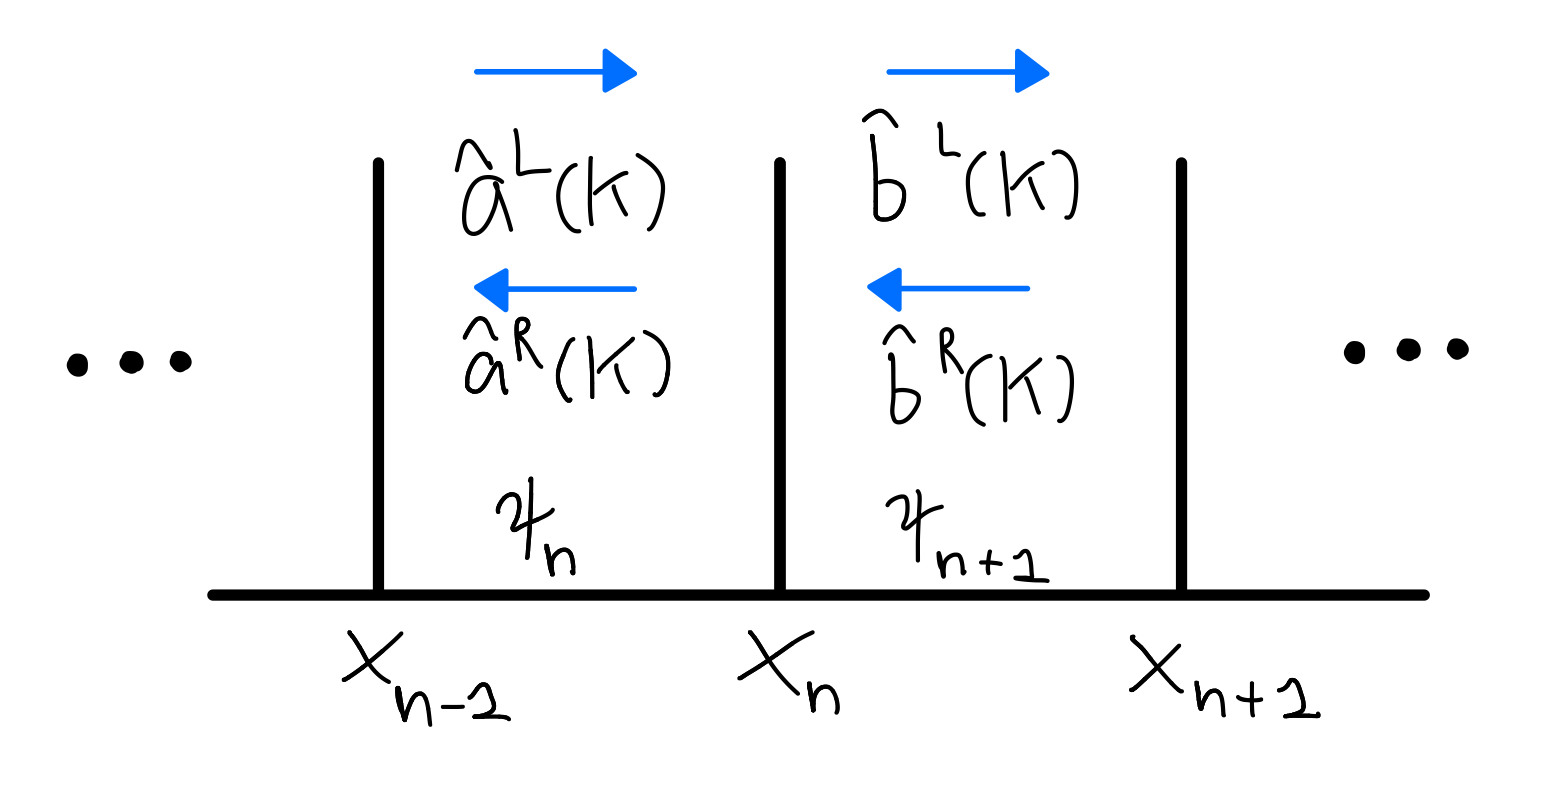
\includegraphics[width=4.5in, keepaspectratio]{figures/boundary_schematic.png}
    \caption{Schematic showing Bloch functions and creation/annihilation operators in the CPWs to the left, and right of SQUID site $n$.}
\end{figure}
%
We use the fact that the Bloch functions $\psi_K(x)$ are, by construction, eigenfunctions of the same boundary condition (see Appendix \ref{ch:appendix_bloch}). Then, we can write our boundary condition in the form
%
\begin{equation}
    \left[\hat{a}^R(K) - \hat{b}^R(K)\right]\left.\frac{\partial \psi^R_K(x)}{\partial x}\right|_{x=n^+}
    +
    \left[\hat{a}^L(K) - \hat{b}^L(K)\right]\left.\frac{\partial \psi^L_K(x)}{\partial x}\right|_{x=n^+} = 0 
\end{equation}
%
Using (eq. \ref{eq:bloch_waves}) and the relation $u_K(x) = u^*_K(x)$ (see Appendix \ref{ch:appendix_bloch}),
%
\begin{equation}\label{eq:BC_static_2}
\begin{split}
    \left[\hat{a}^R(K) - \hat{b}^R(K)\right]\left.\left\lbrace i K \, u_K(x) + \frac{\partial u_K(x)}{\partial x}\right\rbrace\right|_{x=n}\,e^{i K n}
    \\[2mm]
    +
    \left[\hat{a}^L(K) - \hat{b}^L(K)\right]\left.\left\lbrace-i K\, u_K(x) + \frac{\partial u_K(x)}{\partial x}\right\rbrace\right|_{x=n}\,e^{-i K n} = 0 
\end{split}
\end{equation}
%
We now define the short hand notations
%
\begin{gather}
    \mathcal{C}_K = \left.u_K(x)\right|_{x=n}
    \label{eq:cal_C}\\
    %
    \mathcal{D}_K = \left.\frac{\partial u_K(x)}{\partial x}\right|_{x=n}
    \label{eq:cal_D}\\
    %
    \mathcal{A}_K = iK\mathcal{C}_K + \mathcal{D}_K.
    \label{eq:cal_A}
\end{gather}
%
As well as, 
\begin{subequations}\label{eq:cr_an_position_dept}
\begin{eqnarray}
    \hat{a}^R_K(x) = \hat{a}^R(K)\,e^{i K x},
    \\
    \hat{a}^L_K(x) = \hat{a}^L(K)\,e^{-i K x}. 
\end{eqnarray}
\end{subequations}
%
Similarly for $\hat{b}(K)$. We can now write a clean form for our boundary condition using (Eq. \ref{eq:cal_C} - \ref{eq:cr_an_position_dept}),
%
\begin{equation}\label{eq:BC_static_3}
    \left.\left[\hat{a}^R_K(x) - \hat{b}_K^R(x)\right]\right|_{x=n} \mathcal{A}_K
    +
    \left.\left[\hat{a}^L_K(x) - \hat{b}^L_K(x)\right]\right|_{x=n}\mathcal{A}^*_K = 0 
\end{equation}
%
We also impose the requirement that $\hat{\phi}_n(x,\mu)$ is continuous at the boundary $x=n$. Which, using (Eq. \ref{eq:bloch_waves}, we can express as,
%
\begin{equation}\label{eq:continuity_static}
    \left.\left[\hat{a}^R_K(x) + \hat{a}^L_K(x)\right]\right|_{x=n}
    =
    \left.\left[\hat{b}^R_K(x) + \hat{b}^L_K(x)\right]\right|_{x=n}
\end{equation}
%
Using (Eq. \ref{eq:BC_static_3}, \ref{eq:continuity_static}), we arrive at the relations between annihilation coefficients for static applied magnetic flux in our SQUIDs ($E_J(t)= E^0_J$),
%
\begin{subequations}\label{eq:static_solutions}
\begin{eqnarray}
    \hat{b}^R(K) = \hat{a}^R(K),
    \\
    \hat{b}^L(K) = \hat{a}^L(K).
\end{eqnarray}
\end{subequations}
%
Similar equations can be obtained for creation operators by using (Eq. \ref{eq:phi_FT_b}), for $\mu<0$. Note that these solutions are only valid for allowed frequencies $\mu$, given by the band structure of the lattice, i.e. frequencies $\mu$ satisfying (Eq. \ref{eq:bands_condition}). Now that we have obtained solutions for the static case, it is time to analyse the case of an externally driven system.

\section{Weak Harmonic Drive Solution}\label{eq:Static_Flux}

We proceed to drive our system by applying an external flux equally to all of the SQUID sites, such that the form of the time-dependent Josephson energy (Eq. \ref{eq:energyexp1}), where the drive is in phase $\varphi_n=0$ is:
%
\begin{equation}\label{eq:energy_t}
\begin{split}
    E_J(t) = E^0_J + \epsilon(t),
    \\
    \text{where,} \hspace{2mm}
    \epsilon(t) = \delta E^0_J \cos(\Omega t). 
\end{split}
\end{equation}
%
We consider a weak harmonic drive, such that $\frac{\delta E^0_J}{E^0_j} \ll 1$. We can now write the Fourier transformed boundary condition for a time-dependent drive $E_J(t)$. Using our results for the static case (Eq. \ref{eq:BC_static_3}), we can express (Eq. \ref{eq:BC_field}) as a static part plus a dynamic part,
%
Separating the integral in our boundary condition (Eq. \ref{eq:BC_harmonic_drive}) into two sections, (for positive and negative $\mu$), and using (Eq. \ref{eq:cal_C}-\ref{eq:cr_an_position_dept}),

%
\begin{equation}\label{eq:BC_harmonic_drive}
\begin{split}
    \left(\frac{\hbar}{L_0}\right)
    \left|\left.\frac{d\omega}{dK}\right|_{\omega=\mu}\right|^{-1}
    \frac{1}{\sqrt{\mu}}
    \left.
    \left\lbrace
    \left[\hat{a}^R_K(x) - \hat{b}_K^R(x)\right]
    \mathcal{A}_K +
    \left[\hat{a}^L_K(x) - \hat{b}^L_K(x)\right]
    \mathcal{A}^*_K
    \right\rbrace
    \right|_{x=n}
    \\[4mm]
    +\hspace{2mm}
    \hbar \, \left(\frac{2\pi}{\Phi_0}\right)^2
    %
    \left\lbrace
    \int_{0}^{\infty} d \mu'\,
    \delta g(\mu, \mu')
    \left|\left.\frac{d\omega}{dK}\right|_{\omega=\mu'}\right|^{-1}
    \left\lbrace
    \hat{a}^R_K(x) + \hat{a}_K^L(x)
    \right\rbrace
    \mathcal{C}_K\right.
    \\[2mm]
    +
    \left.
    \left.
    \int_{-\infty}^{0} d \mu'\,
    \delta g(\mu, \mu')
    \left|\left.\frac{d\omega}{dK}\right|_{\omega=\mu'}\right|^{-1}
    \left\lbrace
    [\hat{a}^R_K(x)]^\dagger + [\hat{a}_K^L(x)]^\dagger
    \right\rbrace
    \mathcal{C}_K
    \right\rbrace
    \right|_{x=n}
    = 0
    %
\end{split}
\end{equation}
%
Where we have defined:
\begin{gather}\label{eq:Energy_FT}
    \delta g(\mu, \mu') = \frac{1}{2 \pi} \sqrt{\frac{|\mu|}{|\mu'|}}
    \int_{-\infty}^{\infty} dt \, \epsilon(t) \, e^{i(\mu - \mu')t}
    \\
    g(\mu, \mu') = \frac{1}{2 \pi} \sqrt{\frac{|\mu|}{|\mu'|}}
    \int_{-\infty}^{\infty} dt \, E_J(t) \, e^{i(\mu - \mu')t}
    = E_J^0 + \delta g(\mu, \mu').
\end{gather}
%
Which, for a weak harmonic drive $\epsilon(t)$ of the form (Eq. \ref{eq:energy_t}),
%
\begin{equation}
    \delta g(\mu, \mu') = \delta E_J^0
    \left[
    \delta (\mu' - \mu - \Omega) +
    \delta(\mu' - \mu + \Omega)
    \right]
\end{equation}
%
or, in terms of $K$,
\begin{equation}
    \delta g(K,K')= \delta E^0_J
    \left[ 
    d\omega (K'+K_+) \delta (K' - K_+)
    + d\omega (K'-K_-) \delta(K' - K_-)
    \right]
\end{equation}
% 
where we have used the shorthand notations,
%
\begin{gather}
    d\omega (K) =     \left|\left.\frac{d\omega}{dK}\right|_{\omega=\mu}\right|^{-1} 
    \label{eq:shorthand_dw}
    \\
    %
    K_+ = K(\mu + \Omega),\\
    %
    K_- = K(\mu - \Omega).
\end{gather}
%
Making a change of variables to so that integration runs over $K'=K(\mu')$, and separating the integral in our boundary condition (Eq. \ref{eq:BC_harmonic_drive}) into two sections, for ($\mu > 0$) and ($\mu < 0$), and using (Eq. \ref{eq:cr_an_position_dept}, \ref{eq:cal_C}-\ref{eq:cal_A}, and \ref{eq:shorthand_dw}),
%
\begin{equation}\label{eq:BC_harmonic_drive}
\begin{split}
    \left(\frac{\hbar}{L_0}\right)
    \frac{d\omega(K)}{\sqrt{\mu}}
    \left.
    \left\lbrace
    \left[\hat{a}^R_K(x) - \hat{b}_K^R(x)\right]
    \mathcal{A}_K +
    \left[\hat{a}^L_K(x) - \hat{b}^L_K(x)\right]
    \mathcal{A}^*_K
    \right\rbrace
    \right|_{x=n}
    \\[4mm]
    +\hspace{2mm}
    \hbar \, \left(\frac{2\pi}{\Phi_0}\right)^2
    %
    \left[
    \int_{0}^{\infty} dK'\,
    \delta g(K, K')
    d \omega(K')
    \left\lbrace
    \hat{a}^R_K(x) + \hat{a}_K^L(x)
    \right\rbrace
    \mathcal{C}_K\right.
    \\[4mm]
    +
    \left.
    \int_{-\infty}^{0} dK'\,
    \delta g(K, K')
    \left\lbrace
    [\hat{a}^R_K(x)]^\dagger + [\hat{a}_K^L(x)]^\dagger
    \right\rbrace
    \mathcal{C}_K
    \right]
    = 0
    %
\end{split}
\end{equation}